
\subsection{Low-depth (uknown genotypes)}

\begin{frame}
\frametitle{NGS data processing in the \textbf{model} world}

	\begin{figure}
		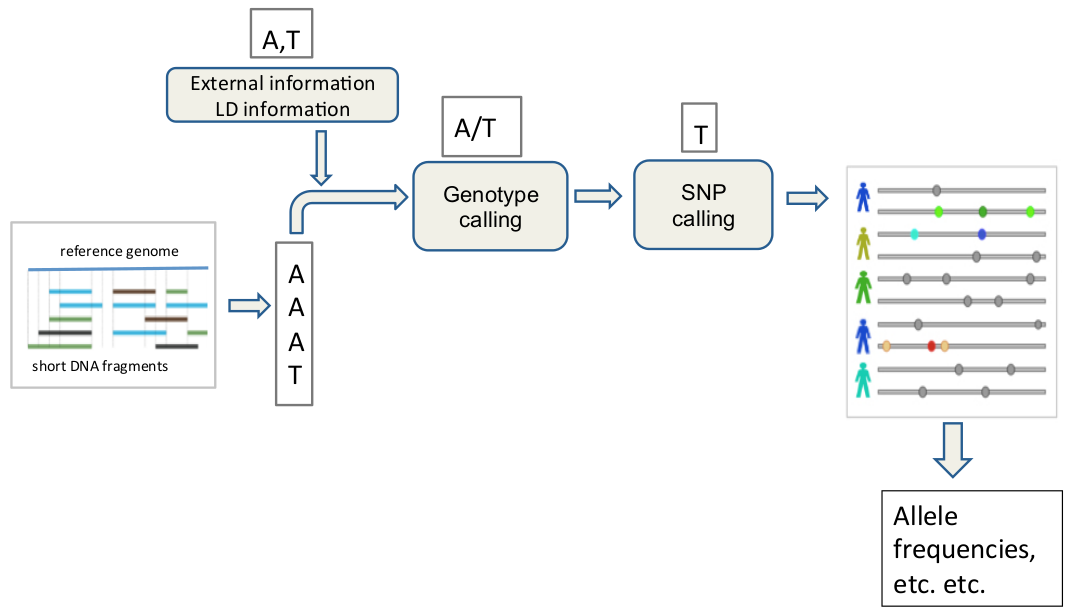
\includegraphics[width=\textwidth]{Pics/ngs_1.png}
	\end{figure}

\end{frame}

\begin{frame}
\frametitle{NGS data processing in the \textbf{non-model} world}

	\begin{figure}
        	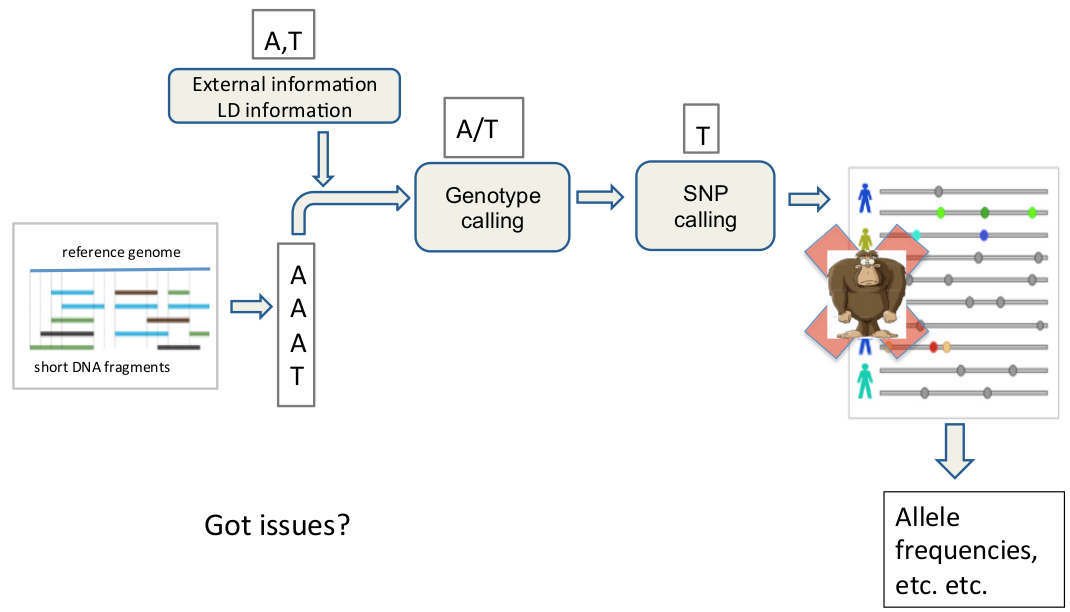
\includegraphics[width=\textwidth]{Pics/ngs_2.png}
	\end{figure}

\end{frame}

\begin{frame}
\frametitle{NGS data processing in the \textbf{non-model} world}

	\begin{figure}
        	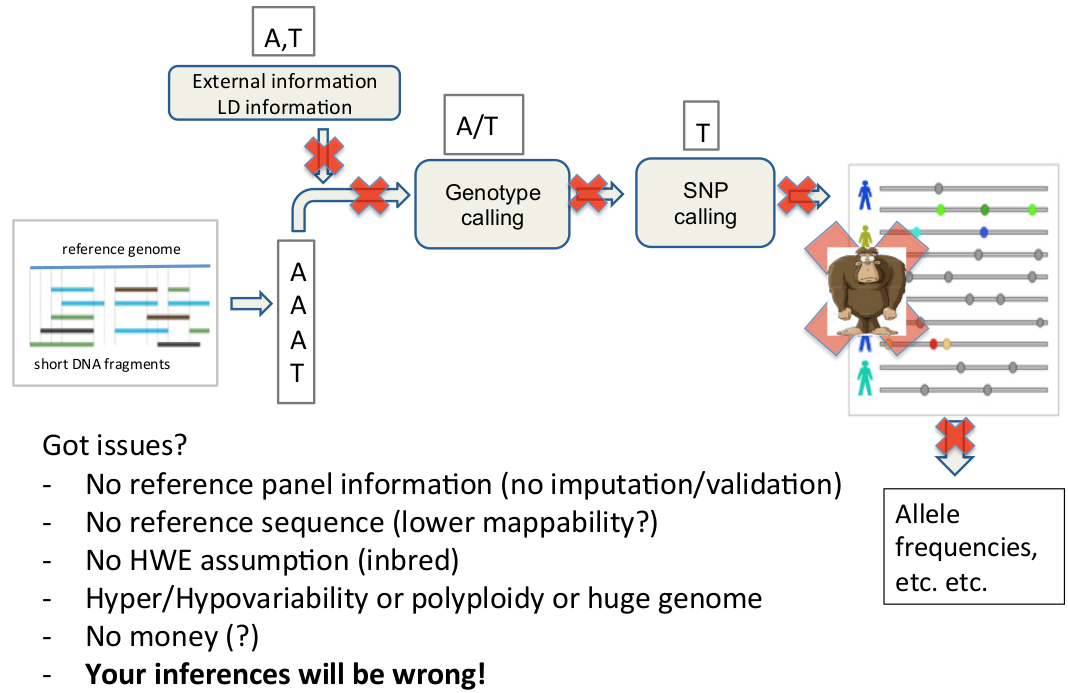
\includegraphics[width=\textwidth]{Pics/ngs_3.png}
	\end{figure}

\end{frame}

\begin{frame}
\frametitle{NGS data processing in the \textbf{non-model} world}

	\begin{figure}
        	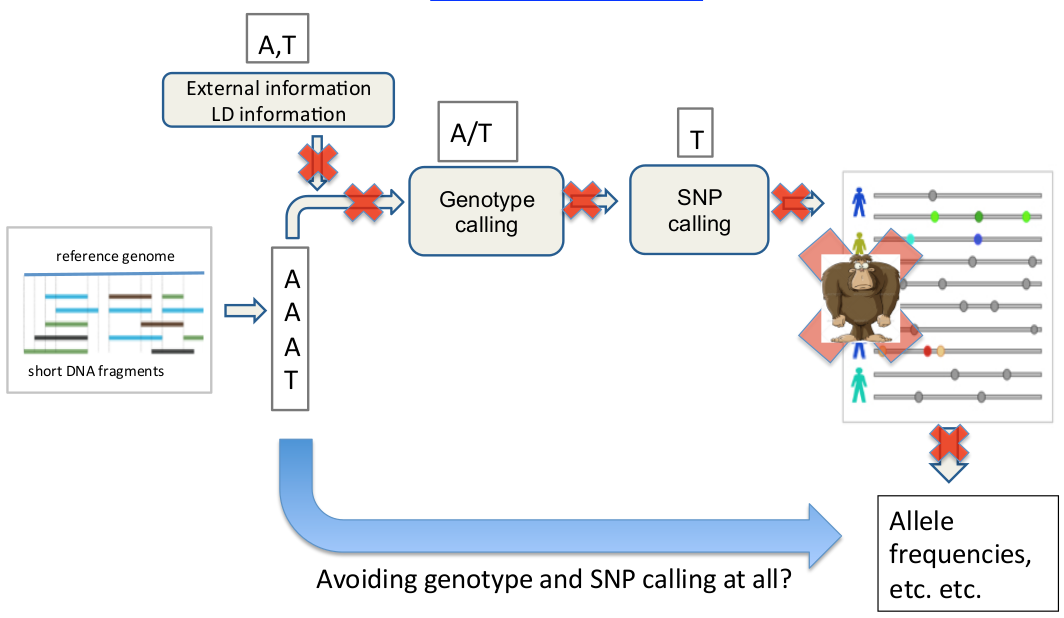
\includegraphics[width=\textwidth]{Pics/ngs_4.png}
	\end{figure}

\end{frame}


%%%%%%%%%%%%%%%%%%%%%%%%%%%%%%%%%%%%%%%%%%%%%%

\begin{frame}
\frametitle{Summary statistics}

	Aim: estimate the number of heterozygotes ($H$) from \textbf{unknown} genotypes.

	Data:
	\begin{center}
                \begin{tabular}{c | c | c | c | c}
                	Sample & Data & $P(G=AA|D)$ & $P(G=AG|D)$ & $P(G=GG|D)$\\
        		\hline
			1 & A & 0.66 & 0.33 & 0.01\\
			2 & AAAG & 0.14 & 0.86 & 0.00\\
			3 & AGG & 0.00 & 0.92 & 0.08\\
			4 & GG & 0.00 & 0.20 & 0.80\\
        		\hline
                \end{tabular}
		with $Q=15$
        \end{center}

	Solutions:
	\begin{enumerate}
		\item call genotypes: $H=2$
		\pause
		\item sample genotypes: $H$ is defined by a distribution 
	\end{enumerate}


\end{frame}

%%%%%%%%%%%%%%%%%%%%%%%%%%%%%%%%%%%%%%%%%%%

\begin{frame}
\frametitle{Summary statistics}

	\tiny{
        \begin{center}
                \begin{tabular}{c | c | c | c | c}
                        Sample & Data & $P(G=AA|D)$ & $P(G=AG|D)$ & $P(G=GG|D)$\\
                        \hline
                        1 & A & 0.66 & 0.33 & 0.01\\
                        2 & AAAG & 0.14 & 0.86 & 0.00\\
                        3 & AGG & 0.00 & 0.92 & 0.08\\
                        4 & GG & 0.00 & 0.20 & 0.80\\
                        \hline
                \end{tabular}
                with $Q=15$
        \end{center}
	}
	
	Sampling genotypes:
	\begin{figure}
		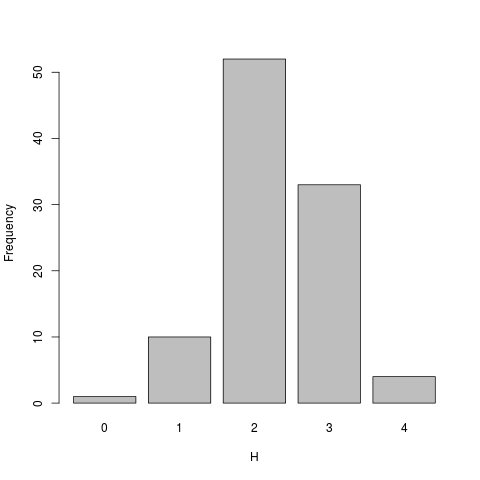
\includegraphics[width=0.45\textwidth]{Pics/H.png}
	\end{figure}


\end{frame}

%%%%%%%%%%%%%%%%%%%%%%%%%%%%%%%%%%%%%%%%%%%%

\begin{frame}
\frametitle{Expected value}

	\begin{figure}
                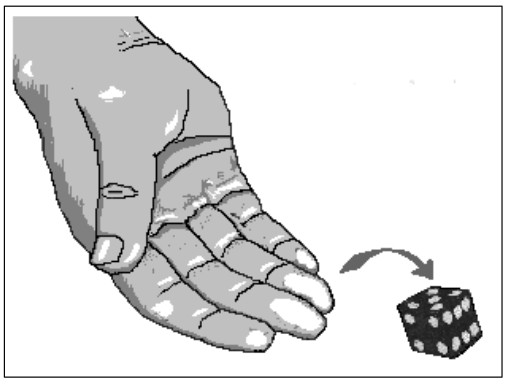
\includegraphics[width=0.5\textwidth]{Pics/die.png}
        \end{figure}

	\begin{itemize}
		\item What are the possible outcomes of this experiment?
		\item With what probability?
	\end{itemize}

\end{frame}

%%%%%%%%%%%%%%%%%%%%%%%%%%%%%%%%%%%%%%%%%%%%

\begin{frame}
\frametitle{Expected value}

	The expected	value	of	a	discrete	random	variable	is	the probability-weighted	average	of	all	possible	values

	\begin{equation*}
		E[X|D] = \sum_{i=1}^N x_i p(X=x_i|D)
	\end{equation*}
	
	\pause

	
		$E[X|D] = 1 \cdot \frac{1}{6} + 2 \cdot \frac{1}{6} + 3 \cdot \frac{1}{6} + 4 \cdot \frac{1}{6} + 5 \cdot \frac{1}{6} +6 \cdot \frac{1}{6} = \frac{(1+2+3+4+5+6)}{6} = \frac{21}{6} = 3.5$

\end{frame}

%%%%%%%%%%%%%%%%%%%%%%%%%%%%%%%%

\begin{frame}
\frametitle{Expected value}

		It is the average value if you perform the same experiment many times.

        	\begin{figure}
                	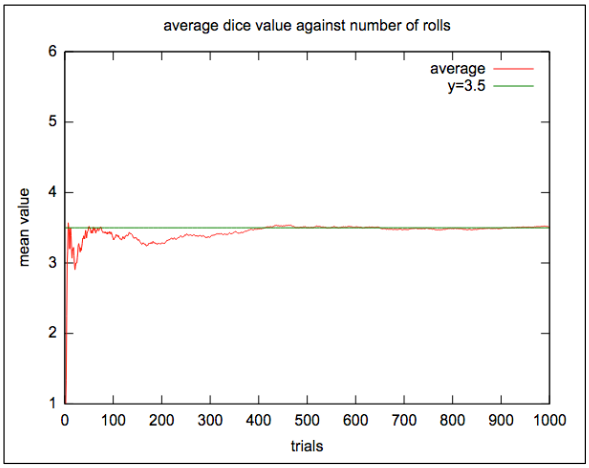
\includegraphics[width=0.5\textwidth]{Pics/die_tries.png}
        	\end{figure}

\end{frame}

%%%%%%%%%%%%%%%%%%%%%%%%%%%%%%%%%%%%%%%%%%%%

\begin{frame}
\frametitle{Summary statistics}

        \tiny{
        \begin{center}
                \begin{tabular}{c | c | c | c | c}
                        Sample & Data & $P(G=AA|D)$ & $P(G=AG|D)$ & $P(G=GG|D)$\\
                        \hline
                        1 & A & 0.66 & 0.33 & 0.01\\
                        2 & AAAG & 0.14 & 0.86 & 0.00\\
                        3 & AGG & 0.00 & 0.92 & 0.08\\
                        4 & GG & 0.00 & 0.20 & 0.80\\
                        \hline
                \end{tabular}
                with $Q=15$
        \end{center}
        }

	\large{
	\begin{enumerate}
                \item call genotypes: $H=2$
                \item sample genotypes: $H$ is defined by a distribution
		\item expected value: $\hat{H}$ = \pause $p(G_1=AG) + p(G_2=AG) + p(G_3=AG) + p(G_4=AG) = 0.33+0.86+0.92+0.20 = 2.31$
        \end{enumerate}
	}

\end{frame}


%%%%%%%%%%%%%%%%%%%%%%%%%%%%%%%%%%%%%%%%%%%%%%%

\begin{frame}
\frametitle{Genetic distances}

	\begin{figure}
                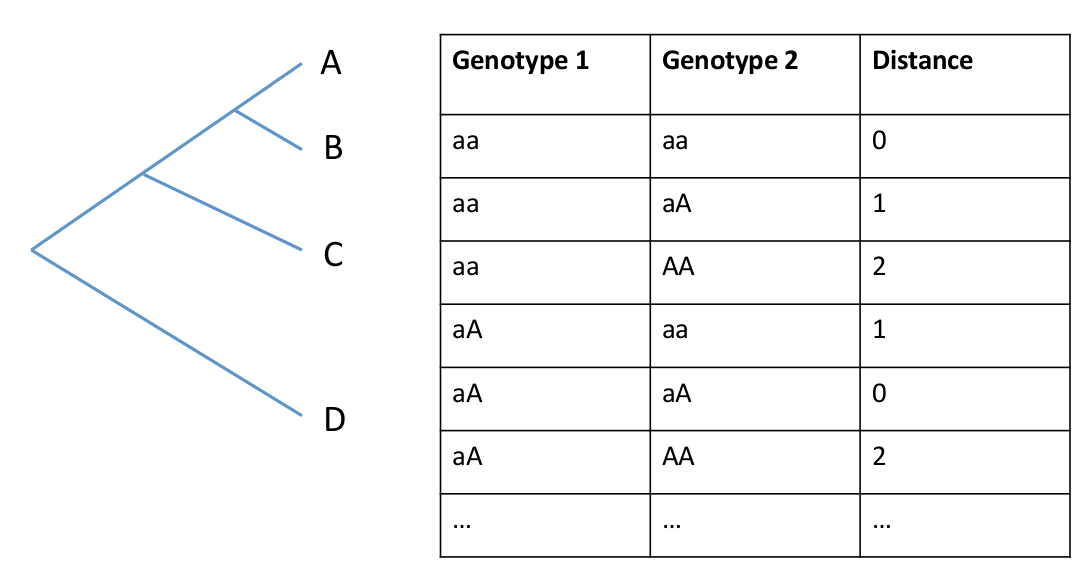
\includegraphics[width=\textwidth]{Pics/gdist_1.png}
        \end{figure}


\end{frame}

%%%%%%%%%%%%%%%%%%%%%%%%%%%%%%%%%%%%%%%%%%%%%%%

\begin{frame}
\frametitle{Genetic distances}

        \begin{figure}
                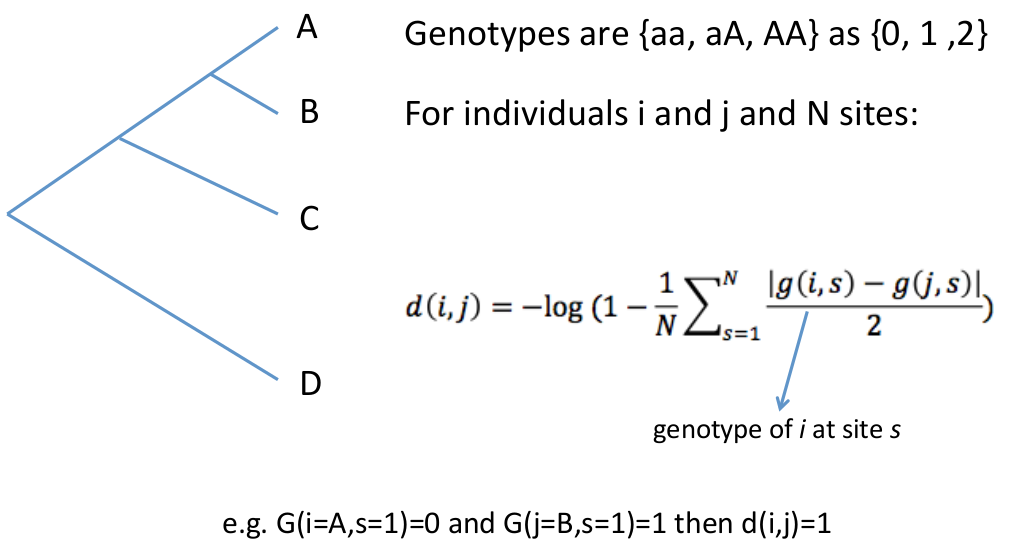
\includegraphics[width=\textwidth]{Pics/gdist_2.png}
        \end{figure}

\end{frame}

%%%%%%%%%%%%%%%%%%%%%%%%%%%%%%%%%%%%%%%%%%%%%%%

\begin{frame}
\frametitle{Genetic distances from known genotypes}

        \begin{figure}
                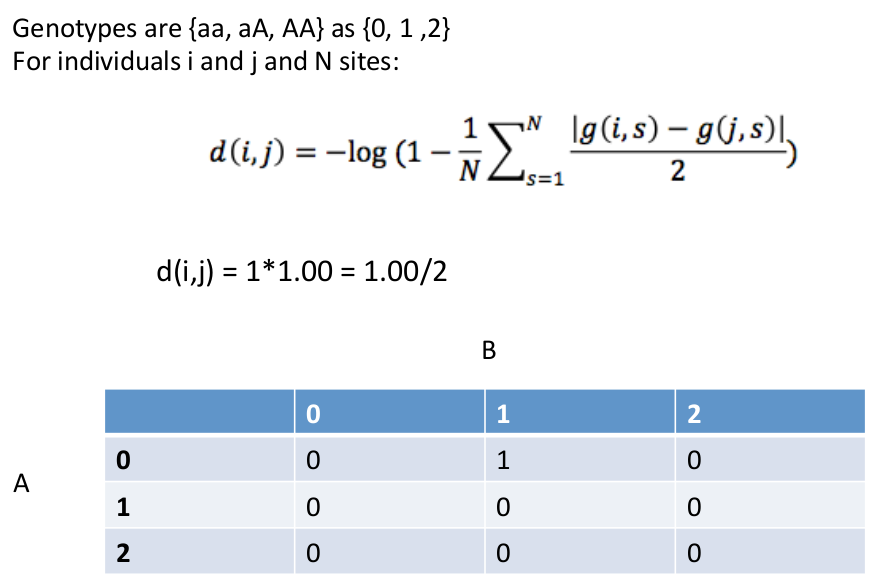
\includegraphics[width=\textwidth]{Pics/gdist_3.png}
        \end{figure}

\end{frame}

%%%%%%%%%%%%%%%%%%%%%%%%%%%%%%%%%%%%%%%%%%%%%%%

\begin{frame}
\frametitle{Genetic distances from \textbf{unknown} genotypes}

        \begin{figure}
                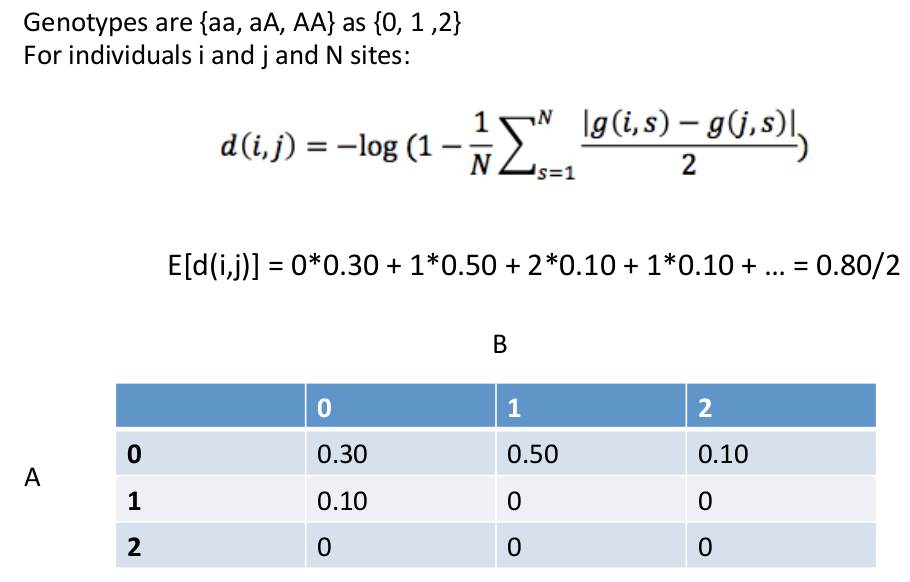
\includegraphics[width=\textwidth]{Pics/gdist_4.png}
        \end{figure}

\end{frame}

%%%%%%%%%%%%%%%%%%%%%%%%%%%%%%%%%%%%%%%%%%%%%%%

\begin{frame}
\frametitle{Genetic distances from \textbf{unknown} genotypes}

        \begin{figure}
                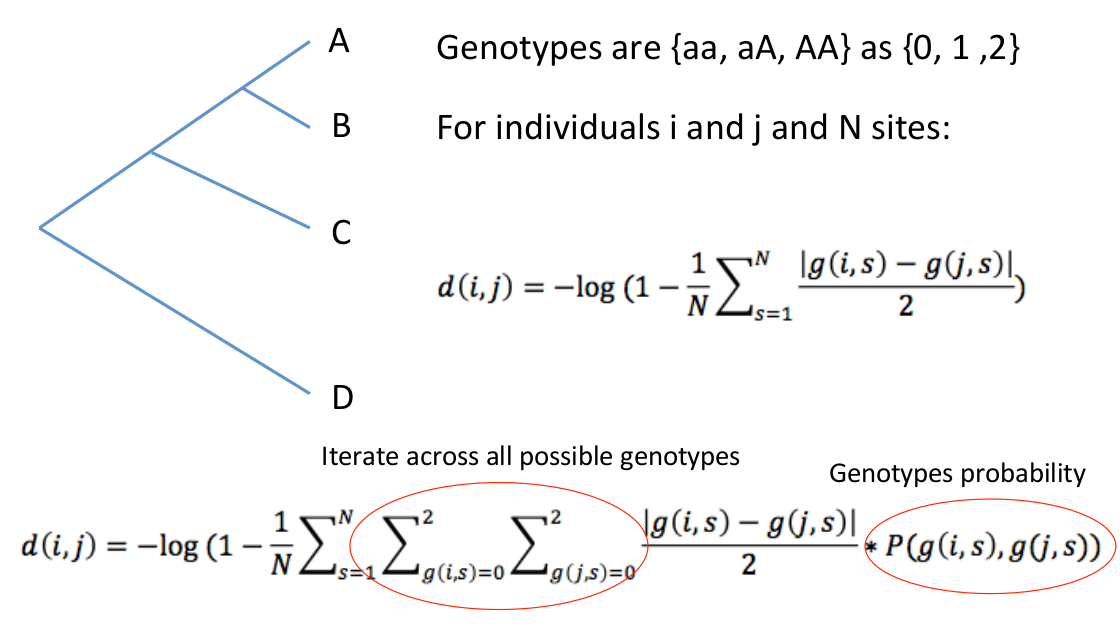
\includegraphics[width=\textwidth]{Pics/gdist_5.png}
        \end{figure}

\end{frame}

%%%%%%%%%%%%%%%%%%%%%%%%%%%%%%%%%%%%%%%%%%%%%%%

\begin{frame}
\frametitle{Genetic distances from \textbf{unknown} genotypes}

        \begin{figure}
                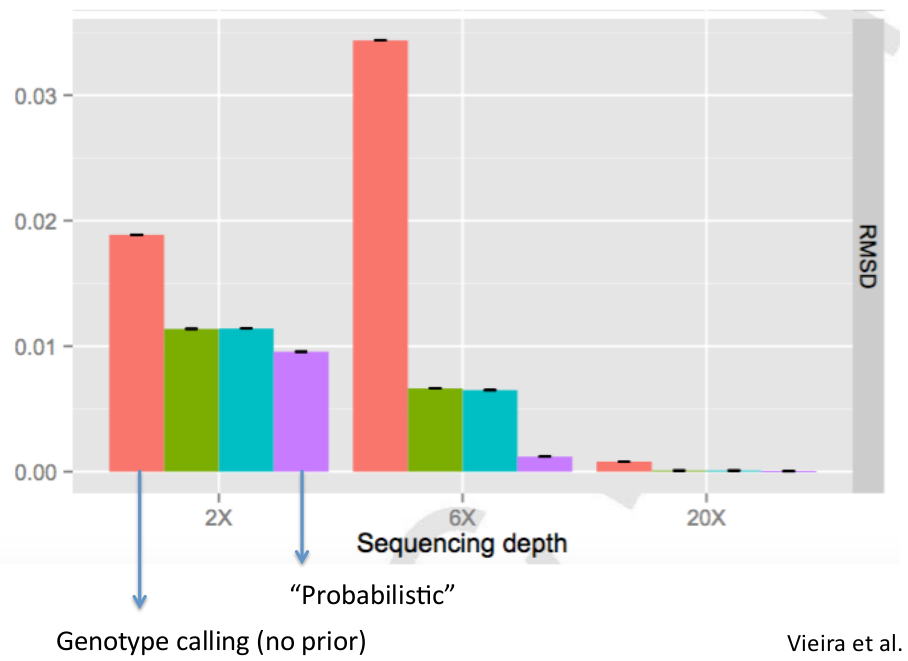
\includegraphics[width=\textwidth]{Pics/gdist_6.png}
        \end{figure}

\end{frame}

%%%%%%%%%%%%%%%%%%%%%%%%%%%%%%%%%%%%%%%%%%%%%%%

\begin{frame}
\frametitle{Clustering from \textbf{unknown} genotypes}

        \begin{figure}
                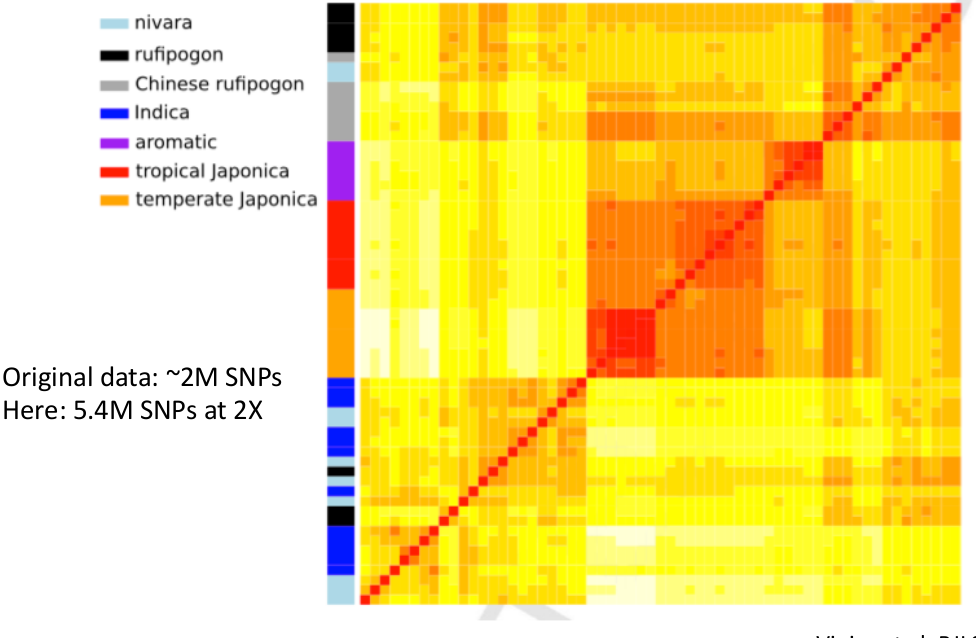
\includegraphics[width=\textwidth]{Pics/gdist_7.png}
        \end{figure}

\end{frame}


%%%%%%%%%%%%%%%%%%%%%%%%%%%%%%%%%%%%%%%%%%%%%

\begin{frame}

	pca

\end{frame}

%%%%%%%%%%%%%%%%%%%%%%%%%%%%%%%%%%%%%%%%%%%%%%%

\begin{frame}
\frametitle{Exercise 2}

	PCA with both methods

	Alone: best PCA with filtering (perhaps later when introducing snp calling)

\end{frame}







